\documentclass[a4paper]{article}
\usepackage[french]{babel}
\usepackage[utf8]{inputenc}
\usepackage{graphicx}
\usepackage{amsmath}
\usepackage{subcaption}
\usepackage[T1]{fontenc}
\usepackage{graphicx}
\usepackage{caption}
\usepackage[colorlinks=true, allcolors=blue]{hyperref}

%%%%%%%%%%%%%%%% Lengths %%%%%%%%%%%%%%%%
\setlength{\textwidth}{16cm}
\setlength{\evensidemargin}{0.3cm}
\setlength{\oddsidemargin}{0.3cm}

%%%%%%%%%%%%%%%% Variables %%%%%%%%%%%%%%%%
\def\projet{2}
\def\titre{Résolution de systèmes linéaires, application à l'équation de la chaleur}
\def\groupe{1}
\def\equipe{5}
\def\responsible{Sarah Dribi Alaoui}
\def\secretary{Corentin Domas}
\def\others{Mohammed Bouhaja, Abderahim Lagraoui}

\begin{document}

%%%%%%%%%%%%%%%% Header %%%%%%%%%%%%%%%%
\noindent\begin{minipage}{0.98\textwidth}
  \vskip 0mm
  \noindent
  { \begin{tabular}{p{7.5cm}}
      {\bfseries \sffamily
        Projet \projet} \\ 
      {\itshape \titre}
    \end{tabular}}
  \hfill 
  \fbox{\begin{tabular}{l}
      {~\hfill \bfseries \sffamily Groupe \groupe\ - Équipe \equipe
        \hfill~} \\[2mm] 
      Responsable : \responsible \\
      Secrétaire : \secretary \\
      Programmeurs : \others
    \end{tabular}}

\end{minipage}

%%%%%%%%%%%%%%%% Main part %%%%%%%%%%%%%%%%

\section{Résolution de systèmes linéaires}

Pour résoudre un système linéaire $A.x = b$, il existe deux approches principales: les méthodes directes et les méthodes itératives. Les méthodes directes sont plus précises mais peuvent être plus coûteuses en termes de temps de calcul et de mémoire, tandis que les méthodes itératives sont plus efficaces pour les systèmes linéaires très grands, mais nécessitent souvent une bonne approximation initiale et une méthode de convergence adaptée. Nous explorons les deux approches dans ce projet, avec la décomposition de $Cholesky$ comme exemple de méthode directe et la méthode du gradient conjugué comme exemple de méthode itérative.

\subsection{Décomposition de Cholesky}

Soit $n$ un entier naturel. On considère $(E) : A.x = b$ un système linéaire où $A$ est une matrice de $S_n^{++}$, l'ensemble des matrices symétriques définies positives de taille
 $n$, et $b$ et $x$ deux vecteurs colonnes de taille $n$.
L'algorithme de $Cholesky$ consiste à factoriser la matrice $A$ sous la forme d’un produit $ T^{T} \cdot T$ où $T$
est une matrice triangulaire inférieure obtenue par les formules suivantes :

\begin{equation*}
t_{i, j} = \left\{
    \begin{array}{cr}
        \rule{0pt}{2.5ex} \sqrt{ a_{i,i} - \sum_{k=1}^{i-1} t_{i,k}^{2}} & \mbox{si } i=j \\
        \rule{0pt}{4ex} \frac{a_{i,j} - \sum_{k=1}^{i-1} t_{i,k}t_{j,k} } {a_{i,i}}& \mbox{si i $\leq$ j}
    \end{array}
\right.
\end{equation*}

\subsubsection{Implémentation de l'algorithme}

La fonction $cholesky(A)$ crée une matrice nulle $T$ de taille $(n,n)$, puis effectue un parcours de la matrice $A$ en la remplissant au fur et à mesure. D'après les formules précédentes, le calcul du coefficient $t_{i,j}$ à chaque itération $i$ se fait en complexité $O(i)$. De plus, le calcul de toutes les colonnes $C_{j}$ avec $i\leq j$ est en complexité $O(\frac{n(n-i)}{2})$. En conclusion, l'algorithme est en complexité $O(\frac{n^{3}}{4})$, soit en complexité cubique.

\subsubsection{Factorisation incomplète}

La factorisation incomplète est une variante de la méthode classique qui consiste à ne pas calculer le coefficient $t_{i,j}$ de la matrice T lorsque le coefficient $a_{i,j}$ de $A$ est nul\footnote{avec $ 0\leq i,j\leq n$}. En conséquence, ces coefficients restent à zéro.

Cette condition fournit une version optimisée de l'algorithme. En effet, la somme présente dans les formules de construction de la matrice triangulaire ne sera calculée que $N_{0}$ fois, où $N_{0}$ est le nombre d'éléments non nuls de la matrice $A$. La nouvelle complexité de l'algorithme est alors en $O(\frac{N_{0}. n^{2}}{2})$, soit en complexité quadratique. On peut alors constater que cette méthode est plus efficace d'un facteur $n$.

\subsection{Génération de matrices symétriques définies positives creuses}

Les matrices symétriques définies positives creuses sont des matrices qui contiennent un certain nombre de coefficients nuls. Elles sont notamment utiles dans le pré-conditionnement des systèmes linéaires. Pour créer de telles matrices, on exploite la propriété selon laquelle une matrice symétrique dont tous les coefficients sont positifs est toujours une matrice définie positive. Ainsi, l'algorithme crée une matrice nulle et la remplit avec des valeurs positives, en veillant à ce que la matrice reste symétrique, jusqu'à atteindre le nombre de termes extra-diagonaux non nuls désiré.


\subsection{Méthode du gradient conjugué}

L'une des méthodes itératives les plus utilisées dans la résolution d'un système d'équation linéaire de type $A.x = b$ est la méthode du gradient conjugué.


Cette méthode consiste à trouver une solution $x$ en minimisant l'erreur relative 
$rsnew$ défini par $rsnew~=~((b-A.x)^{T}(b-A.x))^{\frac{1}{2}}$ d'une manière itérative. Une direction de descente $p=b-Ax$ est choisie comme la première direction de recherche, puis elle est remplacée à chaque étape par une combinaison de la direction précédente et une autre direction $r=r+\beta*p$. La condition d'arrêt de l'algorithme est lorsque $rsnew$ est inférieur à une valeur tolérée d'erreur fixée à $10^{-10}$. On obtient alors une solution optimale.


\subsection{Simulation de la méthode du gradient conjugué}

Afin de bien simuler cette méthode, nous avons implémenté une autre version de l'algorithme qui stocke les valeurs de l'erreur relative de la solution obtenue à chaque itération. La solution théorique fournie par la fonction $linalg.solve$ de la bibliothèque $numpy$ est considérée comme exacte, et sert donc de référence. On considère les trois normes matricielles $\| . \|_{1}$, $\| . \|_{2}$ et $\| . \|_{A}$ définies par:
\[ \| X \|_{1} = \sum_{i=1}^{n} |x_{i}| \hspace{1cm}  \| X \|_{2} = \sqrt{\sum_{i=1}^{n} (x_{i})^{2}} \hspace{1cm}  \| X \|_{A} =  X^{T}AX\]
avec $X$ un vecteur colonne de taille $n$ et $A \in \mathcal{S}_{n}^{++}$.

\begin{figure}[!h] 
  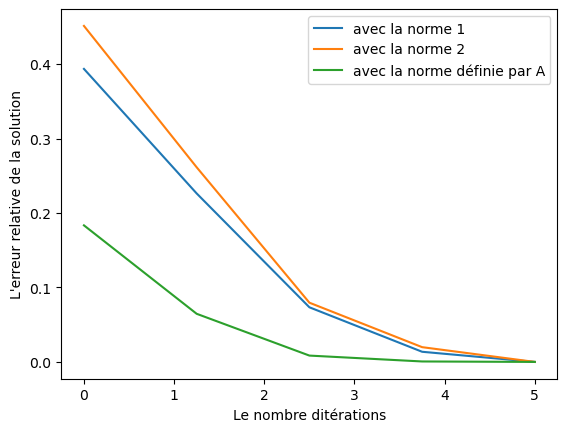
\includegraphics[width=11cm, height= 6.5cm]{normes.png}
  \centering
  \caption{Évaluation de l'erreur relative en fonction de la norme}
  \label{fig:norme}
\end{figure}

La figure \ref{fig:norme} donne l'erreur relative de la méthode en fonction du nombre d'itérations, pour différentes normes. On rappelle, pour une norme $\| \cdot \|$, que l'erreur relative $\delta$ est donnée pour toute matrice $X$ par la formule suivante : 

\begin{equation*}
    \delta(X) = \frac{\|X - X_{sol}\|}{\| X \|}
\end{equation*}

où $X_{sol}$ est la matrice donnée par la méthode de résolution considérée comme exacte.

On constate alors que, quelque soit la norme considérée, l'erreur relative décroît très rapidement de manière exponentielle pour cette méthode. Si on observe une très nette différence pour la norme définie par $A$ sur les premières itérations, elle tend à se résorber dès que le nombre d'itérations augmente.

\subsection{Ajout d'un pré-conditionnement et évaluation de l'erreur}
Un pré-conditionneur $M$ d'une matrice $A$, est une matrice facile à inverser telle que $cond(M^{-1}A$ soit inférieur à $cond(A)$ \textbf{(1)}, où $cond(A)$ est le conditionnement de la matrice $A$. Il sert généralement à optimiser les algorithmes de résolution des systèmes linéaires. Il existe plusieurs méthodes qui génèrent ce type de matrices, à l'aide d'un processus qui peut être itératif ou non itératif. Cependant, nous allons utiliser la matrice $(T^{-1})^{t}T^{-1}$ comme pré-conditionneur, avec $T$ la matrice triangulaire supérieure obtenue par l'algorithme de $cholesky$ appliquée à $A$. 

Afin de vérifier la qualité de ce pré-conditionneur, nous avons réalisé une expérimentation avec un très grand nombre de matrices. Dans tous les cas la condition \textbf{(1)} est vérifiée.

\begin{figure}[!h] 
  \centering
  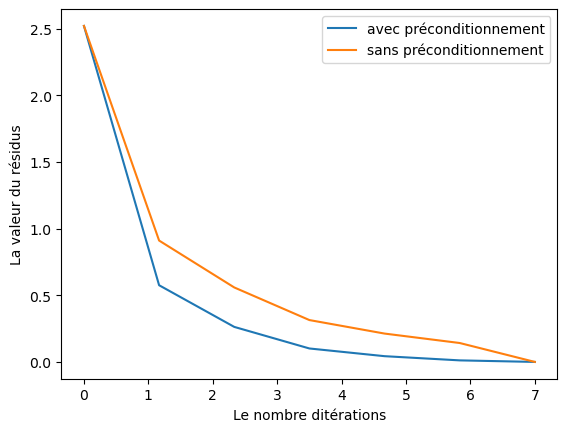
\includegraphics[width=11cm, height= 7cm]{precond.png}
  \caption{Évaluation de l'erreur en fonction du pré-conditionnement}
  \label{fig:precond}
\end{figure}

La figure \ref{fig:precond} représente la valeur du résidu à chaque itération, lors de l'application des deux types de la méthode du gradient conjugué, sur un même problème.

On remarque qu'avec les deux méthodes, la valeur du résidus décroît exponentiellement. Cependant, la méthode qui utilise le pré-conditionnement, tend à faire décroître cette valeur plus rapidement.

%%%%%%%%%%%%%%%%%%%%%%%%%%%%%%%%%%%%%%%%%%%%%%%%%%%%%%%%%%

\section{Application à l'équation de la chaleur}

Le but de cette partie est de résoudre l'équation de la chaleur en utilisant la méthode dite \emph{des différences finies}. 

Considérons une plaque carrée de côté une unité, sur laquelle est définie successivement des conditions initiales et conditions aux limites particulières. La figure \ref{fig:chaleur} donne un résultat de ces simulations, pour différentes méthodes de résolution. Dans cette partie, nous nous intéressons principalement à la méthode de résolution par la méthode du gradient conjugué, ainsi qu'à la méthode de résolution \texttt{linalg} donnée par la bibliothèque \texttt{numpy}, cette dernière servant de référence.

\begin{figure}[!ht]
  $\hspace*{0.6cm}$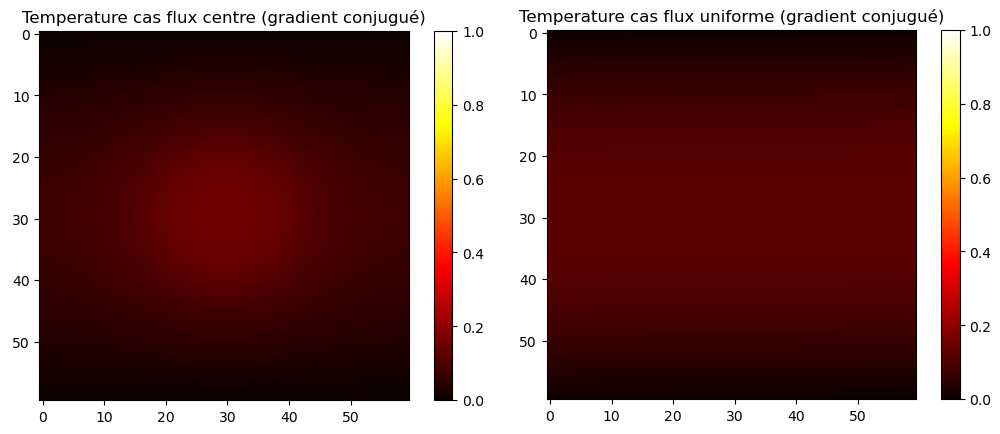
\includegraphics[width=0.9\textwidth]{gc.jpg}
  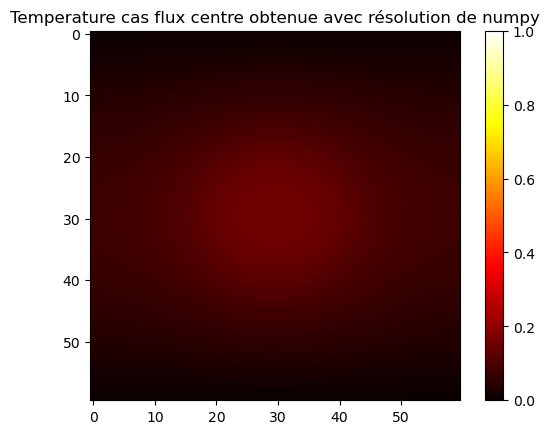
\includegraphics[width=.47\textwidth]{centre-np.png}
  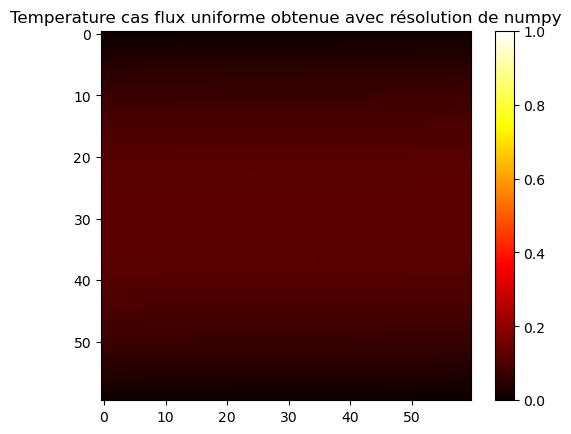
\includegraphics[width=.49\textwidth]{uniforme-np.png}
  \caption{Résolution de l'équation de la chaleur}


  \label{fig:chaleur}
\end{figure}

\subsection{Discrétisation de l'espace}

Nous avons d'abord discrétisé l'espace dans un carré [0;1]×[0,1]. Le nombre de points de la discrétisation spatiale est donné par $N*N$, ceci afin de simplifier la résolution numérique de l'équation \footnote{voir le code python fourni en annexe de ce rapport}.

\subsection{Recherche de $b$ et de $A$}

Une fois ce vecteur représentant les coordonnées spatiales construit,nous lui appliquerons la fonction représentant le flux de la chaleur dépendant des deux dimensions x et y.
Ainsi en mettant un moins,nous avons ainsi obtenu notre vecteur b de taille $N^2$,deuxième membre de l'équation matricielle $AT=b$ ,traduction matricielle de l'équation de la chaleur 

La matrice A n'est que la traduction matricielle de l'opérateur laplacien en utilisant une approximation de la la formule de Taylor à l'ordre 2 et en la combinant avec la discrétisation numérique établie.

Finalement, on obtient un système linéaire qu'il est possible de résoudre avec les méthodes décrites dans la section précédente.

\subsection{Comparaison des profils de température obtenus en 2D}

La figure \ref{fig:chaleur} montre les résultats obtenus en utilisant les deux méthodes de résolution, pour des conditions initiales et conditions aux limites particulières différentes que nous avons conditionné par le choix de deux exemples de flux différents.
On observe alors que les résultats obtenus par la méthode du gradient conjugué et la méthode \texttt{linalg} de \texttt{numpy} sont très similaires, et ne représentent pas d'incohérence avec le principe de diffusion thermique dans chacun des cas.
\footnote{voir le code python fourni en annexe pour plus de détails}

\section*{Conclusion}

En conclusion, l'étude de différentes méthodes de résolution de systèmes linéaires permet de montrer l'efficacité de chacune d'entre elles. Ainsi, nous avons pu explorer les deux grands types de ces algorithmes : ceux de type direct avec l'algorithme de $cholesky$ et ceux qui utilisent des principes itératives avec la méthode du gradient conjugué. Enfin, cette étude nous a également permis d'explorer certains aspects permettant d'optimiser ces algorithmes.

\end{document}
